\section{Gaussian mixture model}
Gaussian mixture model, a.k.a. GMM, or mixture of Gaussians is a mixture model where
\begin{align}
    \vec \alpha                             &\in (0, \infty)^K \\
    \vec \pi \given \alpha                  &\sim \Dir(\vec \alpha) \\
    \vec \mu_k \given \vec m_0, \vec V_0    &\sim \Gauss(\vec m_0, \vec V_0), k = 1, \dotsc, K \\
    \vec \Sigma_k \given \vec S_0, \nu_0    &\sim \IW(\vec S_0, \nu_0), k = 1, \dotsc, K \\
    \vec x_n \given z_n, \vec \theta        &\sim \Gauss\left(\vec \mu_{z_n}, \vec \Sigma_{z_n}\right), n = 1, \dotsc, N
\end{align}
We adopt the following grouping of random variables:
\begin{align}
    \mathcal G_0                            &\coloneqq \left(\vec m_0, \vec V_0, \vec S_0, \nu_0\right) \\
    \vec \theta_k                           &\coloneqq \left(\vec \mu_k, \vec \Sigma_k\right), k = 1, \dotsc, K \\
    \vec \theta                             &\coloneqq (\vec \theta_1, \dotsc, \vec \theta_K).
\end{align}
The graphical model can be seen in Figure~\ref{fig:models/gmm/figures/gmm} below.
\begin{figure}[h!]
    \centering
        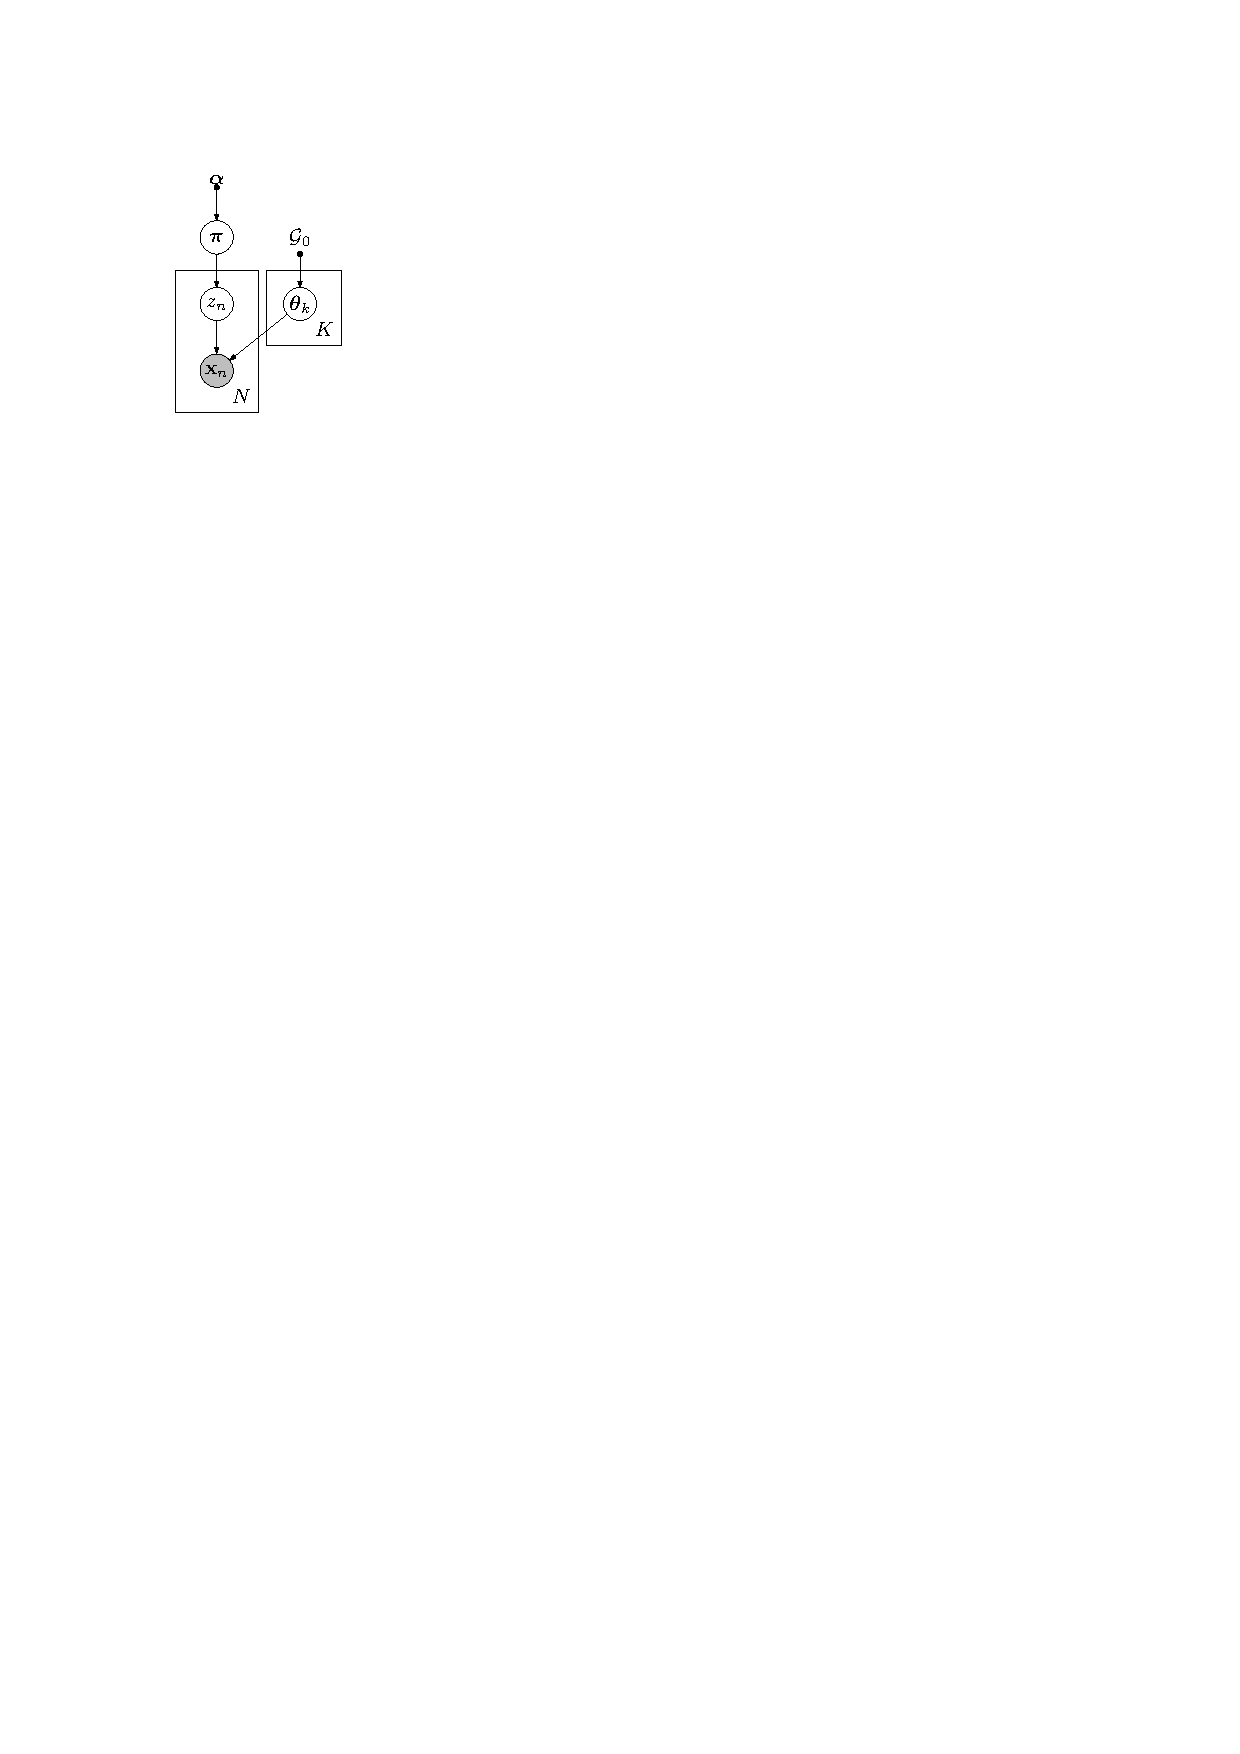
\includegraphics{models/gmm/figures/gmm}
    \label{fig:models/gmm/figures/gmm}
    \caption{Graphical model for the Gaussian mixture model.}
\end{figure}

\subsection{Gibbs sampling for GMMs}
\subsection{Collapsed Gibbs sampling for GMMs}
\subsection{EM algorithm for GMM}
\begin{algorithmbis}[EM algorithm for GMM]\label{alg:models-mm-em-gmm}
    \begin{algorithmic}[1]
        \State Initialise $\vec \theta^{\text{new}} = \left(\left\{\vec \pi_k^{\text{new}}, \vec \mu_k^{\text{new}}, \vec \Sigma_k^{\text{new}}\right\}, k = 1, \dotsc, K\right)$.
        \Repeat
            \State $\vec \theta^{\text{old}} \gets \vec \theta^{\text{new}}$
            \State Set $r_{nk} = p\left(z_n = k \mid \vec x_n; \vec \theta^{\text{old}}\right)$ for $k = 1, \dotsc, K, n = 1, \dotsc, N$. \Comment E step
            \State Set \Comment M step
                \begin{align*}
                    \pi_k^{\text{new}}           &= \frac{\sum_n r_{nk}}{N} \\
                    \vec \mu_k^{\text{new}}      &= \frac{\sum_n r_{nk} \vec x_n}{\sum_n r_{nk}} \\
                    \vec \Sigma_k^{\text{new}}   &= \frac{\sum_n r_{nk}(\vec x_n - \vec \mu_k)(\vec x_n - \vec \mu_k)^T}{\sum_n r_{nk}}
                \end{align*}
                for $k = 1, \dotsc, K$.
        \Until{convergence.}
    \end{algorithmic}
\end{algorithmbis}

The analysis of the algorithm follows.
\paragraph{E step.} We can express $q(\vec Z = \vec K) = p(\vec Z = \vec K \mid \vec X, \vec \theta^{\text{old}})$ where $\vec K = (k_1, \dotsc, k_N), k_n \in \{1, \dotsc, K\}$ for $n =  1, \dotsc, N$ as
\begin{align*}
    p(\vec Z = \vec K \mid \vec X, \vec \theta^{\text{old}})    &= \prod_n p\left(z_n = k_n \mid \vec x_n; \vec \theta^{\text{old}}\right) \\
                                                                &= \prod_n r_{nk_n}\left(\vec \theta^{\text{old}}\right)
\end{align*}
Therefore, in the E step, we set
\begin{equation}
    r_{nk_n}\left(\vec \theta^{\text{old}}\right) = p\left(z_n = k_n \mid \vec x_n; \vec \theta^{\text{old}}\right)
\end{equation}
for $n = 1, \dotsc, N$ for all $\vec K$ and hold it fixed in the M step. This is effectively holding $r_{nk}\left(\vec \theta^{\text{old}}\right)$ (which we will abbreviate as $r_{nk}$ in this section) fixed for $n = 1, \dotsc, N$ and $k = 1, \dotsc, K$.

\paragraph{M step.} We want to find $\vec \theta^{\text{new}} = \argmax_{\vec \theta} \mathcal Q\left(\vec \theta, \vec \theta^{\text{old}}\right)$, where
\begin{align*}
    \mathcal Q\left(\vec \theta, \vec \theta^{\text{old}}\right)    &= \sum_n \sum_k r_{nk} \left(\ln \pi_k + \ln p(\vec x_n \mid z_n = k; \vec \theta)\right)
\end{align*}
To maximise this expression, we use Langrange multipliers because we have a constraint $\sum_k \pi_k = 1$. The Lagrangian is
\begin{equation*}
    \mathcal L_{\mathcal Q}(\vec \theta, \lambda) = \mathcal Q\left(\vec \theta, \vec \theta^{\text{old}}\right) + \lambda \left(1 - \sum_k \pi_k\right)
\end{equation*}
Now, we find the derivatives and set them to zero.

For $\pi_k$,
\begin{align*}
    \frac{\partial \mathcal L_{\mathcal Q}}{\partial \pi_k} &= \frac{\partial}{\partial \pi_k} \left\{\lambda \left(1 - \sum_j \pi_j\right) + \sum_n \sum_j r_{nj} \ln \pi_j\right\} \\
                                                            &= -\lambda + \frac{\sum_n r_{nk}}{\pi_k}
\end{align*}
Setting this to zero, we get
\begin{equation*}
    \pi_k = \frac{\sum_n r_{nk}}{\lambda}
\end{equation*}
but since $\sum_k \pi_k = 1$, we have $\sum_k \frac{\sum_n r_{nk}}{\lambda} = 1$, hence $\lambda = \sum_n \sum_k r_{nk} = \sum_n 1 = N$. Hence
\begin{equation}
    \pi_k = \frac{\sum_n r_{nk}}{N}
\end{equation}
for $k = 1, \dotsc, K$.

For $\vec \mu_k$,
\begin{align*}
    \grad_{\vec \mu_k} \mathcal L_{\mathcal Q}  &= \grad_{\vec \mu_k} \left\{\sum_n \sum_j r_{nj} \left(\ln \pi_j + \ln p(\vec x_n \mid z_n = j; \vec \theta)\right) + \lambda \left(1 - \sum_j \pi_j\right)\right\} \\
                                                &= \grad_{\vec \mu_k} \left\{\sum_n \sum_j r_{nj} \ln \Gauss\left(\vec x_n \mid \vec \mu_j, \vec \Sigma_j\right)\right\} \\
                                                &= \grad_{\vec \mu_k} \left\{\sum_n r_{nk} \ln \Gauss\left(\vec x_n \mid \vec \mu_k, \vec \Sigma_k\right)\right\} \\
                                                &= \grad_{\vec \mu_k} \left\{\sum_n r_{nk} \ln \left[(2\pi)^{-D / 2} |\vec \Sigma_k|^{-1 / 2} \exp{\left(-\frac{1}{2}(\vec x_n - \vec \mu_k)^T \vec \Sigma_k^{-1} (\vec x_n - \vec \mu_k)\right)}\right]\right\} \\
                                                &= \grad_{\vec \mu_k} \left\{\sum_n r_{nk} \left[-\frac{1}{2} \ln |\vec \Sigma_k| - \frac{1}{2}(\vec x_n - \vec \mu_k)^T \vec \Sigma_k^{-1} (\vec x_n - \vec \mu_k)\right]\right\} \\
                                                &= - \sum_n r_{nk} \vec \Sigma_k^{-1}(\vec x_n - \vec \mu_k)
\end{align*}
Setting this to zero, we get
\begin{equation}
    \vec \mu_k = \frac{\sum_n r_{nk} \vec x_n}{\sum_n r_{nk}}
\end{equation}
for $k = 1, \dotsc, K$.

For $\vec \Sigma_k$,
\begin{align*}
    \grad_{\vec \Sigma_k} \mathcal L_{\mathcal Q}   &= \grad_{\vec \Sigma_k} \left\{\sum_n r_{nk} \left[-\frac{1}{2} \ln |\vec \Sigma_k| - \frac{1}{2}(\vec x_n - \vec \mu_k)^T \vec \Sigma_k^{-1} (\vec x_n - \vec \mu_k)\right]\right\} \\
                                                    &= -\frac{1}{2} \sum_n r_{nk} \left[\vec \Sigma_k^{-T} - \vec \Sigma_k^{-T}(\vec x_n - \vec \mu_k)(\vec x_n - \vec \mu_k)^T \vec \Sigma_k^{-T}\right] \\
                                                    &= -\frac{1}{2} \vec \Sigma^{-1} \sum_n r_{nk} \left[\vec I - (\vec x_n - \vec \mu_k)(\vec x_n - \vec \mu_k)^T \vec \Sigma_k^{-1}\right]
\end{align*}
Setting this to zero, we get
\begin{equation}
    \vec \Sigma_k = \frac{\sum_n r_{nk}(\vec x_n - \vec \mu_k)(\vec x_n - \vec \mu_k)^T}{\sum_n r_{nk}}
\end{equation}